% Created by tikzDevice version 0.12.6 on 2026-08-03 03:40:29
% !TEX encoding = UTF-8 Unicode
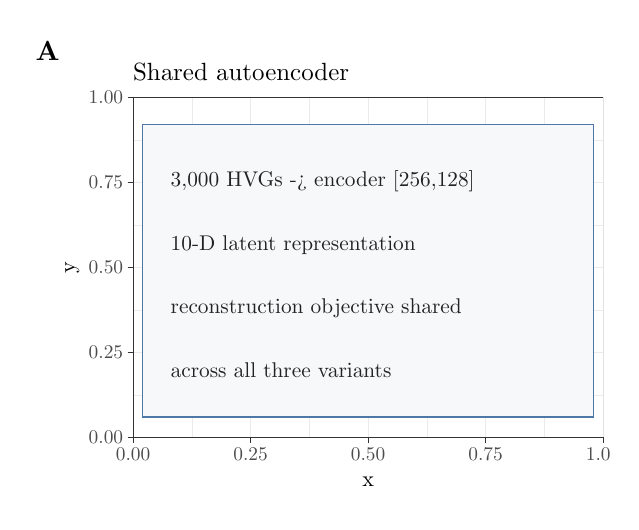
\begin{tikzpicture}[x=1pt,y=1pt]
\definecolor{fillColor}{RGB}{255,255,255}
\path[use as bounding box,fill=fillColor,fill opacity=0.00] (0,0) rectangle (210.78,171.36);
\begin{scope}
\path[clip] (  0.85,  1.87) rectangle (209.93,169.49);
\definecolor{drawColor}{RGB}{255,255,255}
\definecolor{fillColor}{RGB}{255,255,255}

\path[draw=drawColor,line width= 0.4pt,line join=round,line cap=round,fill=fillColor] (  0.85,  1.87) rectangle (209.93,169.49);
\end{scope}
\begin{scope}
\path[clip] ( 38.09, 23.34) rectangle (207.93,146.20);
\definecolor{fillColor}{RGB}{255,255,255}

\path[fill=fillColor] ( 38.09, 23.34) rectangle (207.93,146.20);
\definecolor{drawColor}{gray}{0.92}

\path[draw=drawColor,line width= 0.2pt,line join=round] ( 38.09, 38.69) --
	(207.93, 38.69);

\path[draw=drawColor,line width= 0.2pt,line join=round] ( 38.09, 69.41) --
	(207.93, 69.41);

\path[draw=drawColor,line width= 0.2pt,line join=round] ( 38.09,100.12) --
	(207.93,100.12);

\path[draw=drawColor,line width= 0.2pt,line join=round] ( 38.09,130.84) --
	(207.93,130.84);

\path[draw=drawColor,line width= 0.2pt,line join=round] ( 59.32, 23.34) --
	( 59.32,146.20);

\path[draw=drawColor,line width= 0.2pt,line join=round] (101.78, 23.34) --
	(101.78,146.20);

\path[draw=drawColor,line width= 0.2pt,line join=round] (144.24, 23.34) --
	(144.24,146.20);

\path[draw=drawColor,line width= 0.2pt,line join=round] (186.70, 23.34) --
	(186.70,146.20);

\path[draw=drawColor,line width= 0.4pt,line join=round] ( 38.09, 23.34) --
	(207.93, 23.34);

\path[draw=drawColor,line width= 0.4pt,line join=round] ( 38.09, 54.05) --
	(207.93, 54.05);

\path[draw=drawColor,line width= 0.4pt,line join=round] ( 38.09, 84.77) --
	(207.93, 84.77);

\path[draw=drawColor,line width= 0.4pt,line join=round] ( 38.09,115.48) --
	(207.93,115.48);

\path[draw=drawColor,line width= 0.4pt,line join=round] ( 38.09,146.20) --
	(207.93,146.20);

\path[draw=drawColor,line width= 0.4pt,line join=round] ( 38.09, 23.34) --
	( 38.09,146.20);

\path[draw=drawColor,line width= 0.4pt,line join=round] ( 80.55, 23.34) --
	( 80.55,146.20);

\path[draw=drawColor,line width= 0.4pt,line join=round] (123.01, 23.34) --
	(123.01,146.20);

\path[draw=drawColor,line width= 0.4pt,line join=round] (165.47, 23.34) --
	(165.47,146.20);

\path[draw=drawColor,line width= 0.4pt,line join=round] (207.93, 23.34) --
	(207.93,146.20);
\definecolor{drawColor}{RGB}{78,121,167}
\definecolor{fillColor}{RGB}{247,248,250}

\path[draw=drawColor,line width= 0.5pt,fill=fillColor] ( 41.49, 30.71) rectangle (204.53,136.37);
\definecolor{drawColor}{RGB}{34,34,34}

\node[text=drawColor,anchor=base west,inner sep=0pt, outer sep=0pt, scale=  0.77] at ( 51.68,113.88) {3,000 HVGs -> encoder [256,128]};

\node[text=drawColor,anchor=base west,inner sep=0pt, outer sep=0pt, scale=  0.77] at ( 51.68, 90.94) {10-D latent representation};

\node[text=drawColor,anchor=base west,inner sep=0pt, outer sep=0pt, scale=  0.77] at ( 51.68, 68.01) {reconstruction objective shared};

\node[text=drawColor,anchor=base west,inner sep=0pt, outer sep=0pt, scale=  0.77] at ( 51.68, 45.08) {across all three variants};
\definecolor{drawColor}{gray}{0.20}

\path[draw=drawColor,line width= 0.4pt,line join=round,line cap=round] ( 38.09, 23.34) rectangle (207.93,146.20);
\end{scope}
\begin{scope}
\path[clip] (  0.00,  0.00) rectangle (210.78,171.36);
\definecolor{drawColor}{gray}{0.30}

\node[text=drawColor,anchor=base east,inner sep=0pt, outer sep=0pt, scale=  0.70] at ( 34.49, 20.93) {0.00};

\node[text=drawColor,anchor=base east,inner sep=0pt, outer sep=0pt, scale=  0.70] at ( 34.49, 51.64) {0.25};

\node[text=drawColor,anchor=base east,inner sep=0pt, outer sep=0pt, scale=  0.70] at ( 34.49, 82.36) {0.50};

\node[text=drawColor,anchor=base east,inner sep=0pt, outer sep=0pt, scale=  0.70] at ( 34.49,113.07) {0.75};

\node[text=drawColor,anchor=base east,inner sep=0pt, outer sep=0pt, scale=  0.70] at ( 34.49,143.79) {1.00};
\end{scope}
\begin{scope}
\path[clip] (  0.00,  0.00) rectangle (210.78,171.36);
\definecolor{drawColor}{gray}{0.20}

\path[draw=drawColor,line width= 0.4pt,line join=round] ( 36.09, 23.34) --
	( 38.09, 23.34);

\path[draw=drawColor,line width= 0.4pt,line join=round] ( 36.09, 54.05) --
	( 38.09, 54.05);

\path[draw=drawColor,line width= 0.4pt,line join=round] ( 36.09, 84.77) --
	( 38.09, 84.77);

\path[draw=drawColor,line width= 0.4pt,line join=round] ( 36.09,115.48) --
	( 38.09,115.48);

\path[draw=drawColor,line width= 0.4pt,line join=round] ( 36.09,146.20) --
	( 38.09,146.20);
\end{scope}
\begin{scope}
\path[clip] (  0.00,  0.00) rectangle (210.78,171.36);
\definecolor{drawColor}{gray}{0.20}

\path[draw=drawColor,line width= 0.4pt,line join=round] ( 38.09, 21.34) --
	( 38.09, 23.34);

\path[draw=drawColor,line width= 0.4pt,line join=round] ( 80.55, 21.34) --
	( 80.55, 23.34);

\path[draw=drawColor,line width= 0.4pt,line join=round] (123.01, 21.34) --
	(123.01, 23.34);

\path[draw=drawColor,line width= 0.4pt,line join=round] (165.47, 21.34) --
	(165.47, 23.34);

\path[draw=drawColor,line width= 0.4pt,line join=round] (207.93, 21.34) --
	(207.93, 23.34);
\end{scope}
\begin{scope}
\path[clip] (  0.00,  0.00) rectangle (210.78,171.36);
\definecolor{drawColor}{gray}{0.30}

\node[text=drawColor,anchor=base,inner sep=0pt, outer sep=0pt, scale=  0.70] at ( 38.09, 14.92) {0.00};

\node[text=drawColor,anchor=base,inner sep=0pt, outer sep=0pt, scale=  0.70] at ( 80.55, 14.92) {0.25};

\node[text=drawColor,anchor=base,inner sep=0pt, outer sep=0pt, scale=  0.70] at (123.01, 14.92) {0.50};

\node[text=drawColor,anchor=base,inner sep=0pt, outer sep=0pt, scale=  0.70] at (165.47, 14.92) {0.75};

\node[text=drawColor,anchor=base,inner sep=0pt, outer sep=0pt, scale=  0.70] at (207.93, 14.92) {1.00};
\end{scope}
\begin{scope}
\path[clip] (  0.00,  0.00) rectangle (210.78,171.36);
\definecolor{drawColor}{RGB}{0,0,0}

\node[text=drawColor,anchor=base,inner sep=0pt, outer sep=0pt, scale=  0.80] at (123.01,  5.64) {x};
\end{scope}
\begin{scope}
\path[clip] (  0.00,  0.00) rectangle (210.78,171.36);
\definecolor{drawColor}{RGB}{0,0,0}

\node[text=drawColor,rotate= 90.00,anchor=base,inner sep=0pt, outer sep=0pt, scale=  0.80] at ( 17.05, 84.77) {y};
\end{scope}
\begin{scope}
\path[clip] (  0.00,  0.00) rectangle (210.78,171.36);
\definecolor{drawColor}{RGB}{0,0,0}

\node[text=drawColor,anchor=base west,inner sep=0pt, outer sep=0pt, scale=  0.90] at ( 38.09,152.18) {Shared autoencoder};
\end{scope}
\begin{scope}
\path[clip] (  0.00,  0.00) rectangle (210.78,171.36);
\definecolor{drawColor}{RGB}{0,0,0}

\node[text=drawColor,anchor=base,inner sep=0pt, outer sep=0pt, scale=  1.00] at (  7.20,159.49) {\bfseries A};
\end{scope}
\end{tikzpicture}
